\usetikzlibrary{shapes.geometric, arrows}


\tikzstyle{trait} = [rectangle, rounded corners, minimum width=2cm, minimum height=1cm,text centered, draw=black, fill=white]
\tikzstyle{arrow} = [thick,->,>=stealth]

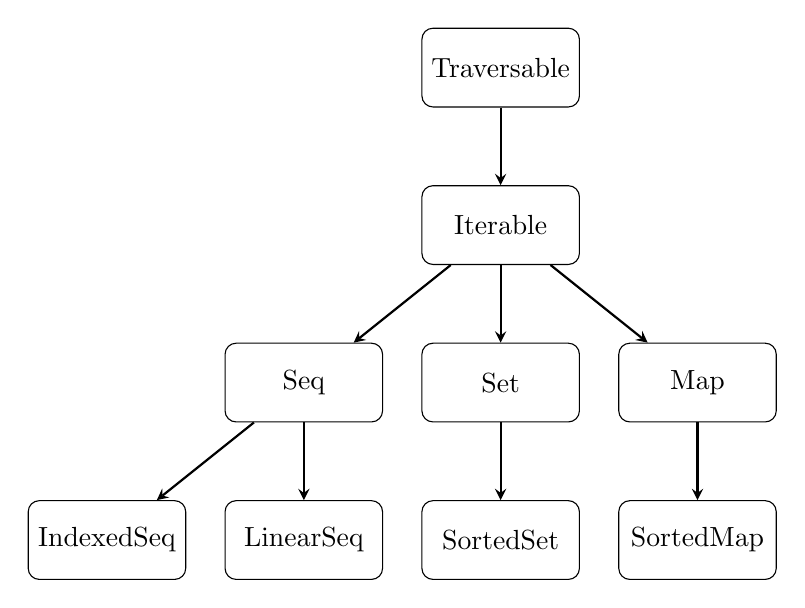
\begin{tikzpicture}[align=center, node distance=2cm]
    \node (traversable) [trait] {Traversable};
    \node (iterable) [trait, below of=traversable] {Iterable};
    \node (set) [trait, below of=iterable] {Set};
    \node (sortedset) [trait, below of=set] {SortedSet};

    \begin{scope}[node distance=25mm]
        \node (seq) [trait, left of=set] {Seq};
        \node (linearseq) [trait, left of=sortedset] {LinearSeq};
        
        \node (map) [trait, right of=set] {Map};
        \node (sortedmap) [trait, right of=sortedset] {SortedMap};
        
        \node (indexedseq) [trait, left of=linearseq] {IndexedSeq};
    \end{scope}

    \draw [arrow] (traversable) -- (iterable);

    \draw [arrow] (iterable) -- (set);
    \draw [arrow] (iterable) -- (seq);
    \draw [arrow] (iterable) -- (map);
    
    \draw [arrow] (seq) -- (indexedseq);
    \draw [arrow] (seq) -- (linearseq);
    
    \draw [arrow] (set) -- (sortedset);

    \draw [arrow] (map) -- (sortedmap);

\end{tikzpicture}